% Options for packages loaded elsewhere
\PassOptionsToPackage{unicode}{hyperref}
\PassOptionsToPackage{hyphens}{url}
%
\documentclass[
  a4paper,
]{article}
\usepackage{amsmath,amssymb}
\usepackage{lmodern}
\usepackage{ifxetex,ifluatex}
\ifnum 0\ifxetex 1\fi\ifluatex 1\fi=0 % if pdftex
  \usepackage[T1]{fontenc}
  \usepackage[utf8]{inputenc}
  \usepackage{textcomp} % provide euro and other symbols
\else % if luatex or xetex
  \usepackage{unicode-math}
  \defaultfontfeatures{Scale=MatchLowercase}
  \defaultfontfeatures[\rmfamily]{Ligatures=TeX,Scale=1}
\fi
% Use upquote if available, for straight quotes in verbatim environments
\IfFileExists{upquote.sty}{\usepackage{upquote}}{}
\IfFileExists{microtype.sty}{% use microtype if available
  \usepackage[]{microtype}
  \UseMicrotypeSet[protrusion]{basicmath} % disable protrusion for tt fonts
}{}
\makeatletter
\@ifundefined{KOMAClassName}{% if non-KOMA class
  \IfFileExists{parskip.sty}{%
    \usepackage{parskip}
  }{% else
    \setlength{\parindent}{0pt}
    \setlength{\parskip}{6pt plus 2pt minus 1pt}}
}{% if KOMA class
  \KOMAoptions{parskip=half}}
\makeatother
\usepackage{xcolor}
\IfFileExists{xurl.sty}{\usepackage{xurl}}{} % add URL line breaks if available
\IfFileExists{bookmark.sty}{\usepackage{bookmark}}{\usepackage{hyperref}}
\hypersetup{
  pdftitle={Heterarchical Control in Sensorimotor Processing},
  pdfauthor={Spencer R. Wilson},
  hidelinks,
  pdfcreator={LaTeX via pandoc}}
\urlstyle{same} % disable monospaced font for URLs
\usepackage[margin=30mm]{geometry}
\usepackage{graphicx}
\makeatletter
\def\maxwidth{\ifdim\Gin@nat@width>\linewidth\linewidth\else\Gin@nat@width\fi}
\def\maxheight{\ifdim\Gin@nat@height>\textheight\textheight\else\Gin@nat@height\fi}
\makeatother
% Scale images if necessary, so that they will not overflow the page
% margins by default, and it is still possible to overwrite the defaults
% using explicit options in \includegraphics[width, height, ...]{}
\setkeys{Gin}{width=\maxwidth,height=\maxheight,keepaspectratio}
% Set default figure placement to htbp
\makeatletter
\def\fps@figure{htbp}
\makeatother
\setlength{\emergencystretch}{3em} % prevent overfull lines
\providecommand{\tightlist}{%
  \setlength{\itemsep}{0pt}\setlength{\parskip}{0pt}}
\setcounter{secnumdepth}{5}

%% pandoc-fignos: required package
\usepackage[capitalise]{cleveref}
\ifluatex
  \usepackage{selnolig}  % disable illegal ligatures
\fi

\title{Heterarchical Control in Sensorimotor Processing}
\author{Spencer R. Wilson}
\date{\today}

\usepackage[capitalise]{cleveref}
\usepackage{graphicx}
\graphicspath{{/Users/spencerw/Google Drive/motor_control/phd/}}
\usepackage{subfigure}

\begin{document}
\maketitle

\hypertarget{internal-model-adaptation-for-linear-quadratic-control}{%
\subsection{Internal Model Adaptation for Linear Quadratic
Control}\label{internal-model-adaptation-for-linear-quadratic-control}}

Here I investigate the effects of approximating internal dynamical
models for movement and using the resulting endpoint error to update
this approximation over trials.

Our state space is denoted \(x\) and our control space \(u\) where
\(dim(x) < dim(u)\). Each trial, we move from state \(x(0)\) to x(N) in
\(N\) timesteps. Each trial, we have a goal state \(x^*\) and a
resulting endpoint error \(e(N) = |x(N) - x^*|^2\).

We use a deterministic linear dynamical system to model our within-trial
state dynamics:

\[
x(t) = Ax(t-1) + Bu(t-1).
\]

For this system, we assume there exists a linear feedback control law
optimal under a given quadratic state and control cost:

\[
u(t) = Kx(t).
\]

We can write the controlled, closed-loop system dynamics for the final
time step \(N\):

\[
\begin{aligned} 
x(N) &= (A - BK)x(N-1) = Cx(N-1) \\
x(N) &= Cx(N-1) = C(Cx(N-2)) \\
x(N) &= C^Nx(0).
\end{aligned} 
\]

where \(C^N\) might be called the trajectory dynamic. If the trajectory
dynamic \(C^N\) is an approximation to the true trajectory dynamic
\(C^{N*}\), we can use the error of a given trajectory to find an
incremental update. The error at the final time step \(N\) for trial
\(r\) is

\[
e(r) = |C^N(r)x(0) - x^*|^2.
\]

This error may be due to several sources. Our internal dynamics model
\(A\) might have error relative to the true dynamic \(A^*\). Our control
gain \(K\) may be optimal relative to our internal model \(A\) but not
with respect to the true dynamic \(A^*\). Finally, we might have an
approximate model \(A\) and a suboptimal control gain \(K\). Note that
since this is still deterministic system, we have yet to include any
source of variability in state or control.

If we assume that our computation of the control gain \(K\) is optimal
for our approximate internal model \(A\) (we can compute a controller
given only our internal representation of the system dynamic being
controlled), we can use our endpoint error to derive a gradient descent
update for \(A\) on trial \(r\):

\[
A(r+1) = A(r) - \eta\frac{\partial{e(r)}}{\partial{A}}
\]

We might think about this as an internal simulation of trial \(r\)'s
trajectory, and a subsequent post hoc evaluation of the movement. To
compute \(\delta\), we must take the gradient with respect to A of the
error:

\[
\begin{aligned}
\frac{\partial{e(r)}}{\partial{A}} &= \frac{\partial{}}{\partial{A}}{|C^N(r)x(0) - x^*|^2}
\end{aligned}
\]

Since the gradient with respect to A is the same as the gradient with
respect to \(C\), we can compute the gradient with respect to C to find:

\[
% 2∑𝑁𝑘=1(𝑀𝑁𝑣−𝑤)𝑇𝑀𝑘−1𝑀𝑁−𝑘𝑣
\frac{\partial{e}}{\partial{A_{ij}}} = 2\sum_{k=1}^N\left[(M^Nx(0) - x^*)^TM^{k-1}\right]_i\left[M^{N-k}x(0)\right]_j
\]

Below is a figure showing LQR simulations across gradient descent
updates to the A matrix after it is corrupted by Gaussian noise. Each
trajectory is a single run of the LQR controlled for 200 time steps. The
star shows the target state, the colored circles show the endpoints of
the trajectories. The red circle is the initial state.

\begin{figure}
\hypertarget{fig:gradient_descent}{%
\centering
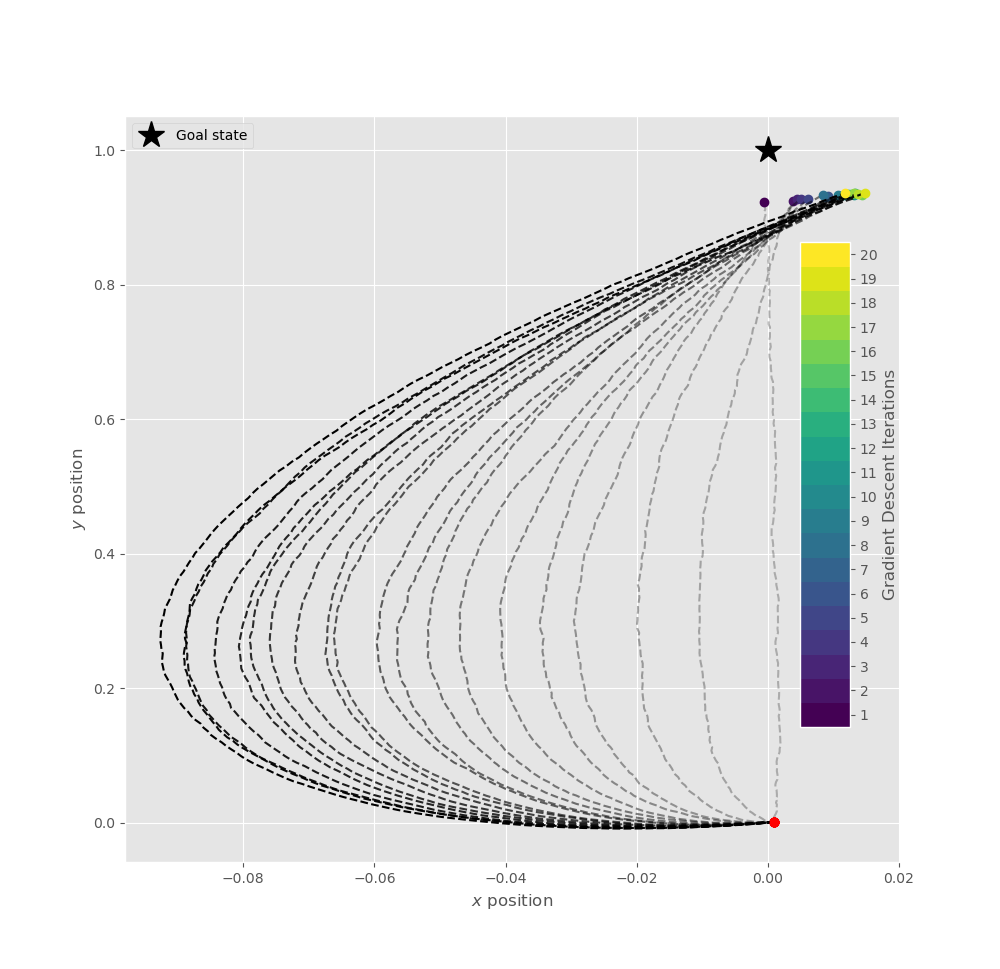
\includegraphics{images/simulations/gradient_descent_on_A.png}
\caption{Iterations of gradient descent on the \(A\) matrix of an
infinite-horizon LQR. Each dotted line in a trajectory with a different
\(A\) matrix. The red circle denotes the initial state, the star denotes
the goal state, and the colored circles denote the endpoints of each
iteration.}\label{fig:gradient_descent}
}
\end{figure}

The descent is converging in endpoint error in position, velocity, and
force space. Unfortunately, this optimization is causing the dynamics to
change. The routine is very fragile to parameter changes. Next steps:

\begin{itemize}
\tightlist
\item
  Corrupt the \(A\) matrix in a more principled way, working to alter
  the passive dynamics in a physically realistic manner.
\item
  Explore the action of the resulting gradient through it's eigenvalues
  and vectors. This can be done in two dimensions as a starting point.
\item
  Compute second-order derivatives and work towards a Newton's method.
\item
  Compute derivatives with respect to the control law \(K\) as a
  comparison.
\item
  Analyze results of the routine in comparison with the reaching
  adaptation literature.
\end{itemize}

\newpage

\hypertarget{bibliography}{%
\subsection{Bibliography}\label{bibliography}}

\end{document}
